% An overview of PostgreSQL
\documentclass[svgnames]{beamer}
\usecolortheme[named=ForestGreen]{structure}
\usetheme{Hannover}
%\usepackage{tipa}
\usepackage{color}
\usepackage{listings}
\usepackage[utf8,latin9]{inputenc}
\usepackage[T1]{fontenc}
%\usepackage{babel}
\beamertemplatenavigationsymbolsempty

\begin{document}
\title{A PostgreSQL Overview}
\author{Joshua Tolley \\ eggyknap \\ End Point Corp.}

\begin{frame}
    
\includegraphics[scale=.45]{Sponsor_slide.png}
\end{frame}

\frame{\titlepage}
%\frame{\tableofcontents}

\section{What is PostgreSQL?}
\begin{frame}
    \begin{itemize}
       \item Began in 1986 under Dr. Michael Stonebraker at U. C. Berkeley as a follow-up to Ingres
       \item Open-sourced in 1996 after its QUEL language was replaced with SQL
       \item Distributed under the PostgreSQL license, similar to the BSD and MIT licenses.
       \item Supports many platforms and operating systems
       \item Large and active community, including several support companies and commercial forks
       \item Designed for extensibility, stability, scalability, and compliance with standards
       \item Currently maintained by volunteer developers worldwide, and a six-person core team
       \item Exceptionally well documented
       \item No single organization owns PostgreSQL
    \end{itemize}
\end{frame}

\section{How does it work?}
\begin{frame}
    \begin{itemize}
        \item Process-based, not thread-based. Communication between processes occurs using various OS-level locking structures and shared memory.
        \begin{columns}[t]
            \begin{column}{0.45\textwidth}
                Advantages
                \begin{itemize}
                    \item Simpler programming. Problems on one backend can't as easily mess up other backends
                    \item Easier to support many architectures
                \end{itemize}
            \end{column}
            \begin{column}{0.45\textwidth}
                Disadvantages
                \begin{itemize}
                    \item Longer startup times for new connections (use a pooler)
                    \item Shared memory applications are particularly slow on Windows; UNIX systems don't have that problem
                \end{itemize}
            \end{column}
        \end{columns}
    \end{itemize}
\end{frame}

\begin{frame}
    \begin{itemize}
        \item ACID-compliant transactions (Atomicity, Consistency, Isolation, Durability)
        \item Multi-version concurrency control
        \begin{itemize}
            \item Some systems (Oracle, MySQL's InnoDB) use a redo log; PostgreSQL stores multiple versions of a row within the table itself
            \item Each row version is marked with transaction IDs to determine its visibility
            \item "Vacuum" cleans out rows that are too old to be visible
            \item ROLLBACK becomes very fast this way; vacuuming and table bloat are notable concerns
        \end{itemize}
    \end{itemize}
\end{frame}

\section{Getting started}
\subsection{Initialization, startup}
%\begin{frame}[fragile]
%\tiny
%        \begin{verbatim}
%initdb initializes a PostgreSQL database cluster.
%
%Usage:
%  initdb [OPTION]... [DATADIR]
%
%Options:
%  -A, --auth=METHOD         default authentication method for local connections
% [-D, --pgdata=]DATADIR     location for this database cluster
%  -E, --encoding=ENCODING   set default encoding for new databases
%      --locale=LOCALE       set default locale for new databases
%      --lc-collate=, --lc-ctype=, --lc-messages=LOCALE
%      --lc-monetary=, --lc-numeric=, --lc-time=LOCALE
%                            set default locale in the respective category for
%                            new databases (default taken from environment)
%      --no-locale           equivalent to --locale=C
%      --pwfile=FILE         read password for the new superuser from file
%  -T, --text-search-config=CFG
%                            default text search configuration
%  -U, --username=NAME       database superuser name
%  -W, --pwprompt            prompt for a password for the new superuser
%  -X, --xlogdir=XLOGDIR     location for the transaction log directory
%
%Less commonly used options:
%  -d, --debug               generate lots of debugging output
%  -L DIRECTORY              where to find the input files
%  -n, --noclean             do not clean up after errors
%  -s, --show                show internal settings
%
%Other options:
%  -?, --help                show this help, then exit
%  -V, --version             output version information, then exit
%
%If the data directory is not specified, the environment variable PGDATA
%is used.
%
%Report bugs to <pgsql-bugs@postgresql.org>.
%        \end{verbatim}
%\normalsize
%\end{frame}

\begin{frame}[fragile]
\small
    \begin{verbatim}
josh@eddie:~/tmp/pgsql$ initdb -D data -U josh
The files belonging to this database system will be owned
by user "josh". This user must also own the server process.
                        
The database cluster will be initialized with locale
en_US.UTF-8. The default database encoding has
accordingly been set to UTF8.

...

WARNING: enabling "trust" authentication for local
connections. You can change this by editing pg_hba.conf
or using the -A option the next time you run initdb.

Success. You can now start the database server using:

    postgres -D data
or  
    pg_ctl -D data -l logfile start
    \end{verbatim}
\normalsize
\end{frame}

\begin{frame}[fragile]
\small
\begin{verbatim}
josh@eddie:~/tmp/pgsql$ pg_ctl -D data/ -l logfile start
server starting         
josh@eddie:~/tmp/pgsql$ cat logfile 
LOG:  autovacuum launcher started
LOG:  database system is ready to accept connections
\end{verbatim}
The initdb application creates a postgres database. When \texttt{pg\_ctl} starts
PostgreSQL, on UNIX it opens a socket, and on Windows it listens on TCP 5432.
\normalsize
\end{frame}

\subsection{Clients}
\begin{frame}[fragile]
psql is a command-line client application that ships with the PostgreSQL code itself
\begin{verbatim}
josh@eddie:~/tmp/pgsql$ psql postgres
psql (9.0.0)
Type "help" for help.

5433 josh@postgres# 
\end{verbatim}
psql features online documentation, tab completion and readline support (are you listening, Oracle?), many simple keyboard commands for manipulating queries and loading instructions from outside the session
\end{frame}

\begin{frame}
For those who prefer a GUI, other options exist, notably PgAdminIII.
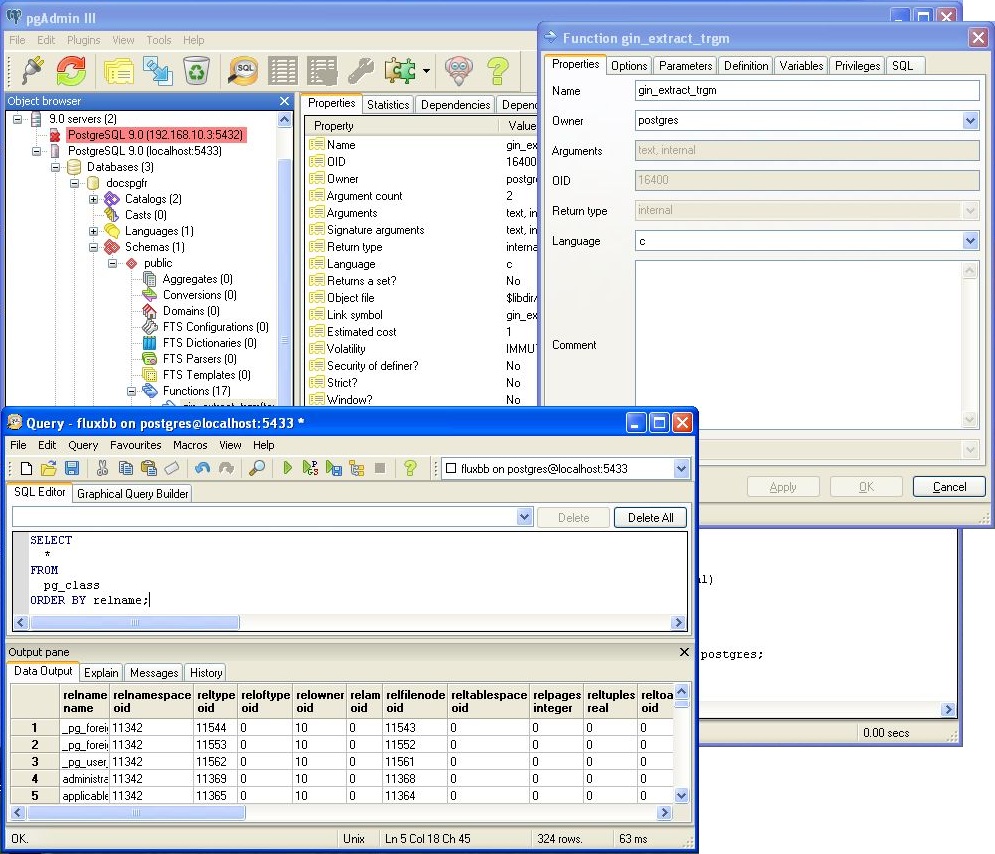
\includegraphics[width=\textwidth]{pgadmin3_win32.png}
\end{frame}

\section{Features}
\subsection{Integrity constraints}
\begin{frame}[fragile]
PostgreSQL correctly handles input validation, triggers, data integrity constraints
\begin{itemize}
    \item NOT NULL
    \item DEFAULT values
    \item Foreign and unique keys
    \item Full, mature trigger support
    \item Correct three-valued logic (i.e. True != False != NULL)
\end{itemize}
Why this might matter:
\small
\begin{verbatim}
mysql> SELECT user_id, expire_date FROM users
WHERE user_id = 1710001;
+---------+-------------+
| user_id | expire_date |
+---------+-------------+
| 1710001 | 0390-08-00  | 
+---------+-------------+
1 row in set (0.05 sec)
\end{verbatim}
\normalsize
\end{frame}

\subsection{Complex queries}
\begin{frame}
PostgreSQL's query parser supports very complex queries without irritating workarounds.
\begin{itemize}
    \item Subqueries
    \item Set operations (INTERSECT, UNION)
    \item Standard SQL operators (COALESCE, CASE, NULLIF)
    \item Arrays
    \item Window functions
    \item Recursive queries
\end{itemize}
\end{frame}

\begin{frame}[fragile]
    Rank employees in each department by salary
    \begin{verbatim}
SELECT first, last, salary, department,
    RANK() OVER (
        PARTITION BY department
        ORDER BY salary DESC
    )
FROM employee
    \end{verbatim}
\end{frame}

\begin{frame}[fragile]
    ... and get this:
    \footnotesize
    \begin{verbatim}
 first  |   last   | salary |   department   | rank
--------+----------+--------+----------------+------
 john   | doe      |  99000 | administration |    1
 speedy | gonzales |  96000 | development    |    1
 hans   | reiser   |  93000 | development    |    2
 martha | stewart  |  90000 | development    |    3
 fred   | rogers   |  97000 | sales          |    1
 carly  | fiorina  |  95000 | sales          |    2
 johnny | carson   |  89000 | sales          |    3
(7 rows)
    \end{verbatim}
    \normalsize
\end{frame}

\begin{frame}[fragile]
    Recursive query to retrieve management hierarchy:
    \begin{verbatim}
# WITH RECURSIVE t (id, managernames) AS (
    SELECT e.id, first || ' ' || last
        AS managernames
    FROM employee e WHERE manager IS NULL
        UNION ALL
    SELECT e.id,
    first || ' ' || last || ', ' || managernames
        AS managernames
    FROM employee e
    JOIN t ON (e.manager = t.id)
    WHERE manager IS NOT NULL
)
SELECT e.id, first || ' ' || last AS name,
    managernames
FROM employee e JOIN t ON (e.id = t.id);
    \end{verbatim}
\end{frame}

\begin{frame}[fragile]
    ...and get this...
    \begin{verbatim}
 id |     name        |  managernames                   
----+-----------------+-----------------------------
  1 | john doe        | john doe
  2 | fred rogers     | fred rogers, john doe
  3 | speedy gonzales | speedy gonzales, john doe
  4 | carly fiorina   | carly fiorina, john doe
  5 | hans reiser     | hans reiser, fred rogers,
    |                 |  john doe
  6 | johnny carson   | johnny carson, hans reiser,
    |                 |  fred rogers, john doe
  7 | martha stewart  | martha stewart, speedy
    |                 |  gonzales, john doe
(7 rows)
    \end{verbatim}
\end{frame}

\begin{frame}[fragile]
    \tiny
    \begin{verbatim}
WITH RECURSIVE x(i) AS
(VALUES(0) UNION ALL SELECT i + 1 FROM x WHERE i < 101),
Z(Ix, Iy, Cx, Cy, X, Y, I)
AS (
    SELECT Ix, Iy, X::float, Y::float, X::float, Y::float, 0
    FROM (SELECT -2.2 + 0.031 * i, i FROM x) AS xgen(x,ix)
        CROSS JOIN
    (SELECT -1.5 + 0.031 * i, i FROM x) AS ygen(y,iy)
        UNION ALL
    SELECT
        Ix, Iy, Cx, Cy, X * X - Y * Y + Cx AS X,
        Y * X * 2 + Cy, I + 1
    FROM Z
    WHERE X * X + Y * Y < 16.0 AND I < 27),
Zt (Ix, Iy, I) AS (
    SELECT Ix, Iy, MAX(I) AS I
    FROM Z GROUP BY Iy, Ix
    ORDER BY Iy, Ix
)
SELECT array_to_string(
    array_agg(
        SUBSTRING(' .,,,-----++++%%%%@@@@#### ',
            GREATEST(I,1), 1)
    ),''
)
FROM Zt GROUP BY Iy ORDER BY Iy;
    \end{verbatim}
    \normalsize
    (yes, this query is SQL-spec compliant)
\end{frame}

\begin{frame}
    \scalebox{.54}{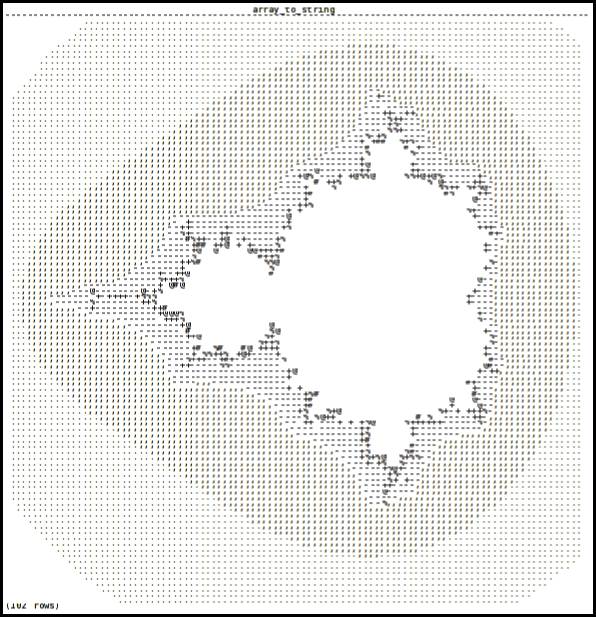
\includegraphics{mandelbrot2.png}}
    %\scalebox{.3}{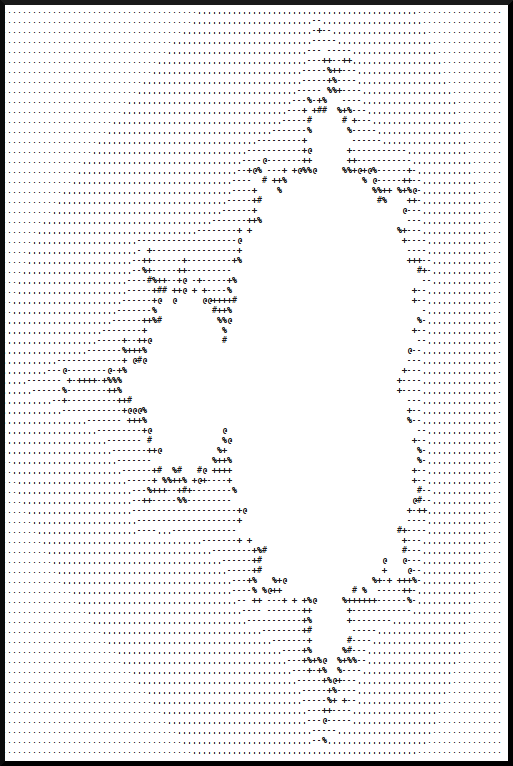
\includegraphics{mandelbrot.png}}
\end{frame}

% outline:
% introductory blabber
% start with initdb
% - introduce "cluster"
% - Everything lives in this directory (unless you make it more complicated)
% - pg_ctl controls this
% psql
% - Each connection starts a new process. Use a connection pooler
% - pg_get_backend_pid()
% - There's also pgadmin (screenshot?)
% Create schemas and views, do some permissions magic
% - Perhaps just show off bits of TriSano
% Describe MVCC, and how a transaction actually works
% - locking, at least. Perhaps kill a session mid-transaction
% - Might as well talk about vacuum and what it is, since folks have heard of it

\subsection{Extensibility}
\begin{frame}
PostgreSQL allows users to customize the database in many different ways:
\begin{itemize}
    \item Functions (including custom aggregates and window functions)
    \item Data types
    \item Index types
    \item Text search configurations (dictionaries, parsers, etc.)
    \item Procedural langauges
    \item Query planners
    \item All sorts of miscellaneous hooks within the backend
\end{itemize}
\end{frame}

\begin{frame}
PostgreSQL offers many "procedural languages" for writing database functions. Four ship with the software by default.
\begin{itemize}
    \item PL/pgSQL (resembles Oracle's PL/SQL)
    \item PL/Perl
    \item PL/Python
    \item PL/Tcl
\end{itemize}
Additionally, many others are available from other sources
\begin{itemize}
    \item PL/Ruby
    \item PL/Java
    \item PL/Scheme
    \item PL/Lua
    \item PL/PHP
    \item PL/R
    \item PL/LOLCODE
\end{itemize}
\end{frame}

\begin{frame}[fragile]
\tiny
\begin{verbatim}
5433 josh@postgres# DO $$
HAI
    BTW Calculate pi using Gregory-Leibniz series
    BTW This method does not converge particularly quickly...
    I HAS A PIADD ITZ 0.0
    I HAS A PISUB ITZ 0.0
    I HAS A ITR ITZ 0
    I HAS A T1
    I HAS A T2
    I HAS A PI ITZ 0.0
    I HAS A ITERASHUNZ ITZ 1000

    IM IN YR LOOP
        T1 R QUOSHUNT OF 4.0 AN SUM OF 3.0 AN ITR
        T2 R QUOSHUNT OF 4.0 AN SUM OF 5.0 AN ITR
        PISUB R SUM OF PISUB AN T1
        PIADD R SUM OF PIADD AN T2
        ITR R SUM OF ITR AN 4.0
        BOTH SAEM ITR AN BIGGR OF ITR AN ITERASHUNZ, O RLY?
            YA RLY, GTFO
        OIC
    IM OUTTA YR LOOP
    PI R SUM OF 4.0 AN DIFF OF PIADD AN PISUB
    VISIBLE "PI R: "
    VISIBLE PI
    FOUND YR PI
KTHXBYE
$$ LANGUAGE PLLOLCODE;
NOTICE:  3.143589
DO
\end{verbatim}
\end{frame}

\begin{frame}
Several useful data types ship with PostgreSQL, or are available from the community.
\begin{itemize}
    \item Geometry and geography data (PostGIS outclasses all open source and most commercial GIS databases)
    \item Network data types (cidr, inet, macaddr)
    \item Array types
    \item User-definable composite types
    \item Intervals
\end{itemize}
Various projects have built very specialized data types using PostgreSQL, for storing such things as probability distributions, mammography images, and gene sequences
\end{frame}

% Show a complex query (bucardo_rate, perhaps?)
% --=< More complex stuff >=--
% Replication
% - Talk about async vs. sync, various available options
% - PITR, hot standby, streaming replication, synchronous replication
% Query planning
% - Mention different join algorithms. Query planner is really complex
% Functions
% - All kinds of PLs, including C
% - Contrib
% - PostGIS (mention some of the bits it's built from)
% Text search
% Window functions
% CTEs
% - Incl. recursion. Mandelbrot example

\subsection{Mission-critical}
\begin{frame}
PostgreSQL functions very well within mission-critical environments, and is widely used by large enterprises:
\begin{itemize}
    \item Afilias, the world's second largest internet registrar, uses PostgreSQL to run their domain name database
    \item Skype uses PostgreSQL as their main database platform
    \item MyYearbook.com, rated in the top 10 social networking sites worldwide in terms of unique visitors, uses PostgreSQL for most everything
    \item Nippon Telegraph and Telepone uses PostgreSQL heavily
    \item Etsy runs their e-commerce site on PostgreSQL
    \item NASA is working on using PostgreSQL in the space station
\end{itemize}
\end{frame}

\begin{frame}
Replication comes in many forms:
\begin{itemize}
    \item Hot standby: built into PostgreSQL, allows read-only slave databases asynchronously updated from a single master
    \item Bucardo: trigger-based replication system allows asynchronous multi-master replication
    \item Slony, Londiste: trigger-based master-slave replication
\end{itemize}
Work is underway to introduce synchronous replication in PostgreSQL 9.1
\end{frame}

\section{Questions?}
\begin{frame}
    
\includegraphics[scale=.25]{logo.png}
\\ Questions?
\end{frame}

\end{document}
